%!TEX root = ../thesis.tex
%*******************************************************************************
%****************************** Third Chapter **********************************
%*******************************************************************************
\chapter{Design}
\graphicspath{{Chapter5/Figs/Raster/}{Chapter5/Figs/Tex/}{Chapter5/Figs/}}

Following the discussion in Chapter 2.3.1 and 2.5, the designs for this project
will be created on top of Hyperledger Fabric, a public permissioned blockchain.
It has become clear that a blockchain specific, high-fidelity prototyping tool is needed
to create system designs such as data models and transactions.

\section{Design Tool}

Hyperledger Composer is an open source development toolset and framework that aims to
accelerate time to value for blockchain projects. It offers business-centric
abstractions, allowing business owners and developers to rapidly develop
use cases and model a blockchain network. The design tools offered take the forms of:
\begin{itemize}
	\setlength\itemsep{0em}
	\item An object-oriented modelling language (.cto file) to define data models in
	      the blockchain network
	\item JavaScript functions (.js file) to define logic for Smart Contracts triggered by transactions
	\item An access control language (.acl file) to define access rules for records on the blockchain\\
	      \citep{official2018composer}
\end{itemize}

See Figure \ref{fig:composer2fabric} for a visual explainer of how Hyperledger Composer
helps designers and developers create these high level definitions.

\begin{figure}[!ht]
	\centering
	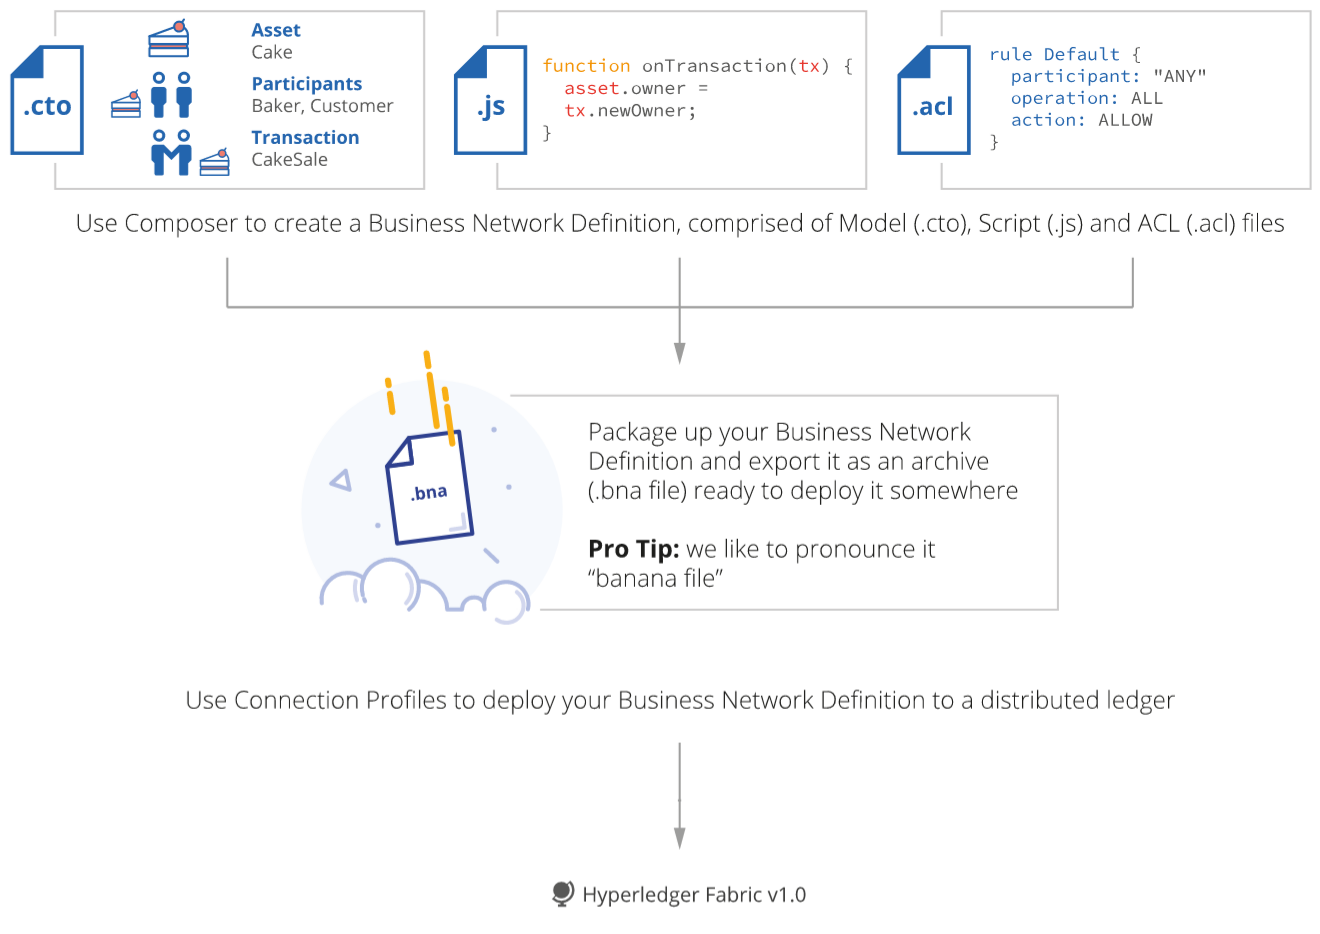
\includegraphics[width=1.0\textwidth]{composer2fabric}
	\caption[Hyperledger Composer]
	{Components in the Hyperledger Composer framework and how it deploys to
		Hyperledger Fabric \citep{cuicapuza2017composer}}
	\label{fig:composer2fabric}
\end{figure}
% https://medium.com/@RichardCuica/hyperledgers-fabric-composer-simplifying-business-networks-on-blockchain-94313b979671

A significant advantage of using Hyperledger Composer is its ability to package these
prototype definitions and deploy it to Hyperledger Fabric, our target blockchain platform.
This will speed up the implementation of the proposed demonstrator applications
in the next stage.

Throughout the design process, the Hyperledger Composer notations are converted or drawn into UML sequence
diagrams, class diagrams and flowcharts. PlantUML, an open source language-to-diagram drawing tool, 
and TikZ, a LaTeX package that creates graphic elements, were used.

The discussion below may regularly refer back to the functional requirements (FR) and
non-functional requirements (NR) defined in the previous Chapter 4.

\section{Transaction Sequences}

A transaction is the only activity that a peer can perform to alter the state of a blockchain.
Designing the sequences of transactions necessary to fulfil the desired user journeys will
be able to provide a good overview of the work ahead. It will also shine a light on 
what data objects and properties must be defined. Two overarching use cases are considered:
assessment and curriculum personalisation.

\subsection{Assessment Use Case}

These four transactions are required to complete the assessment use case (see Figure \ref{fig:assessmentloop}):

\begin{figure}[!ht]
	\centering
	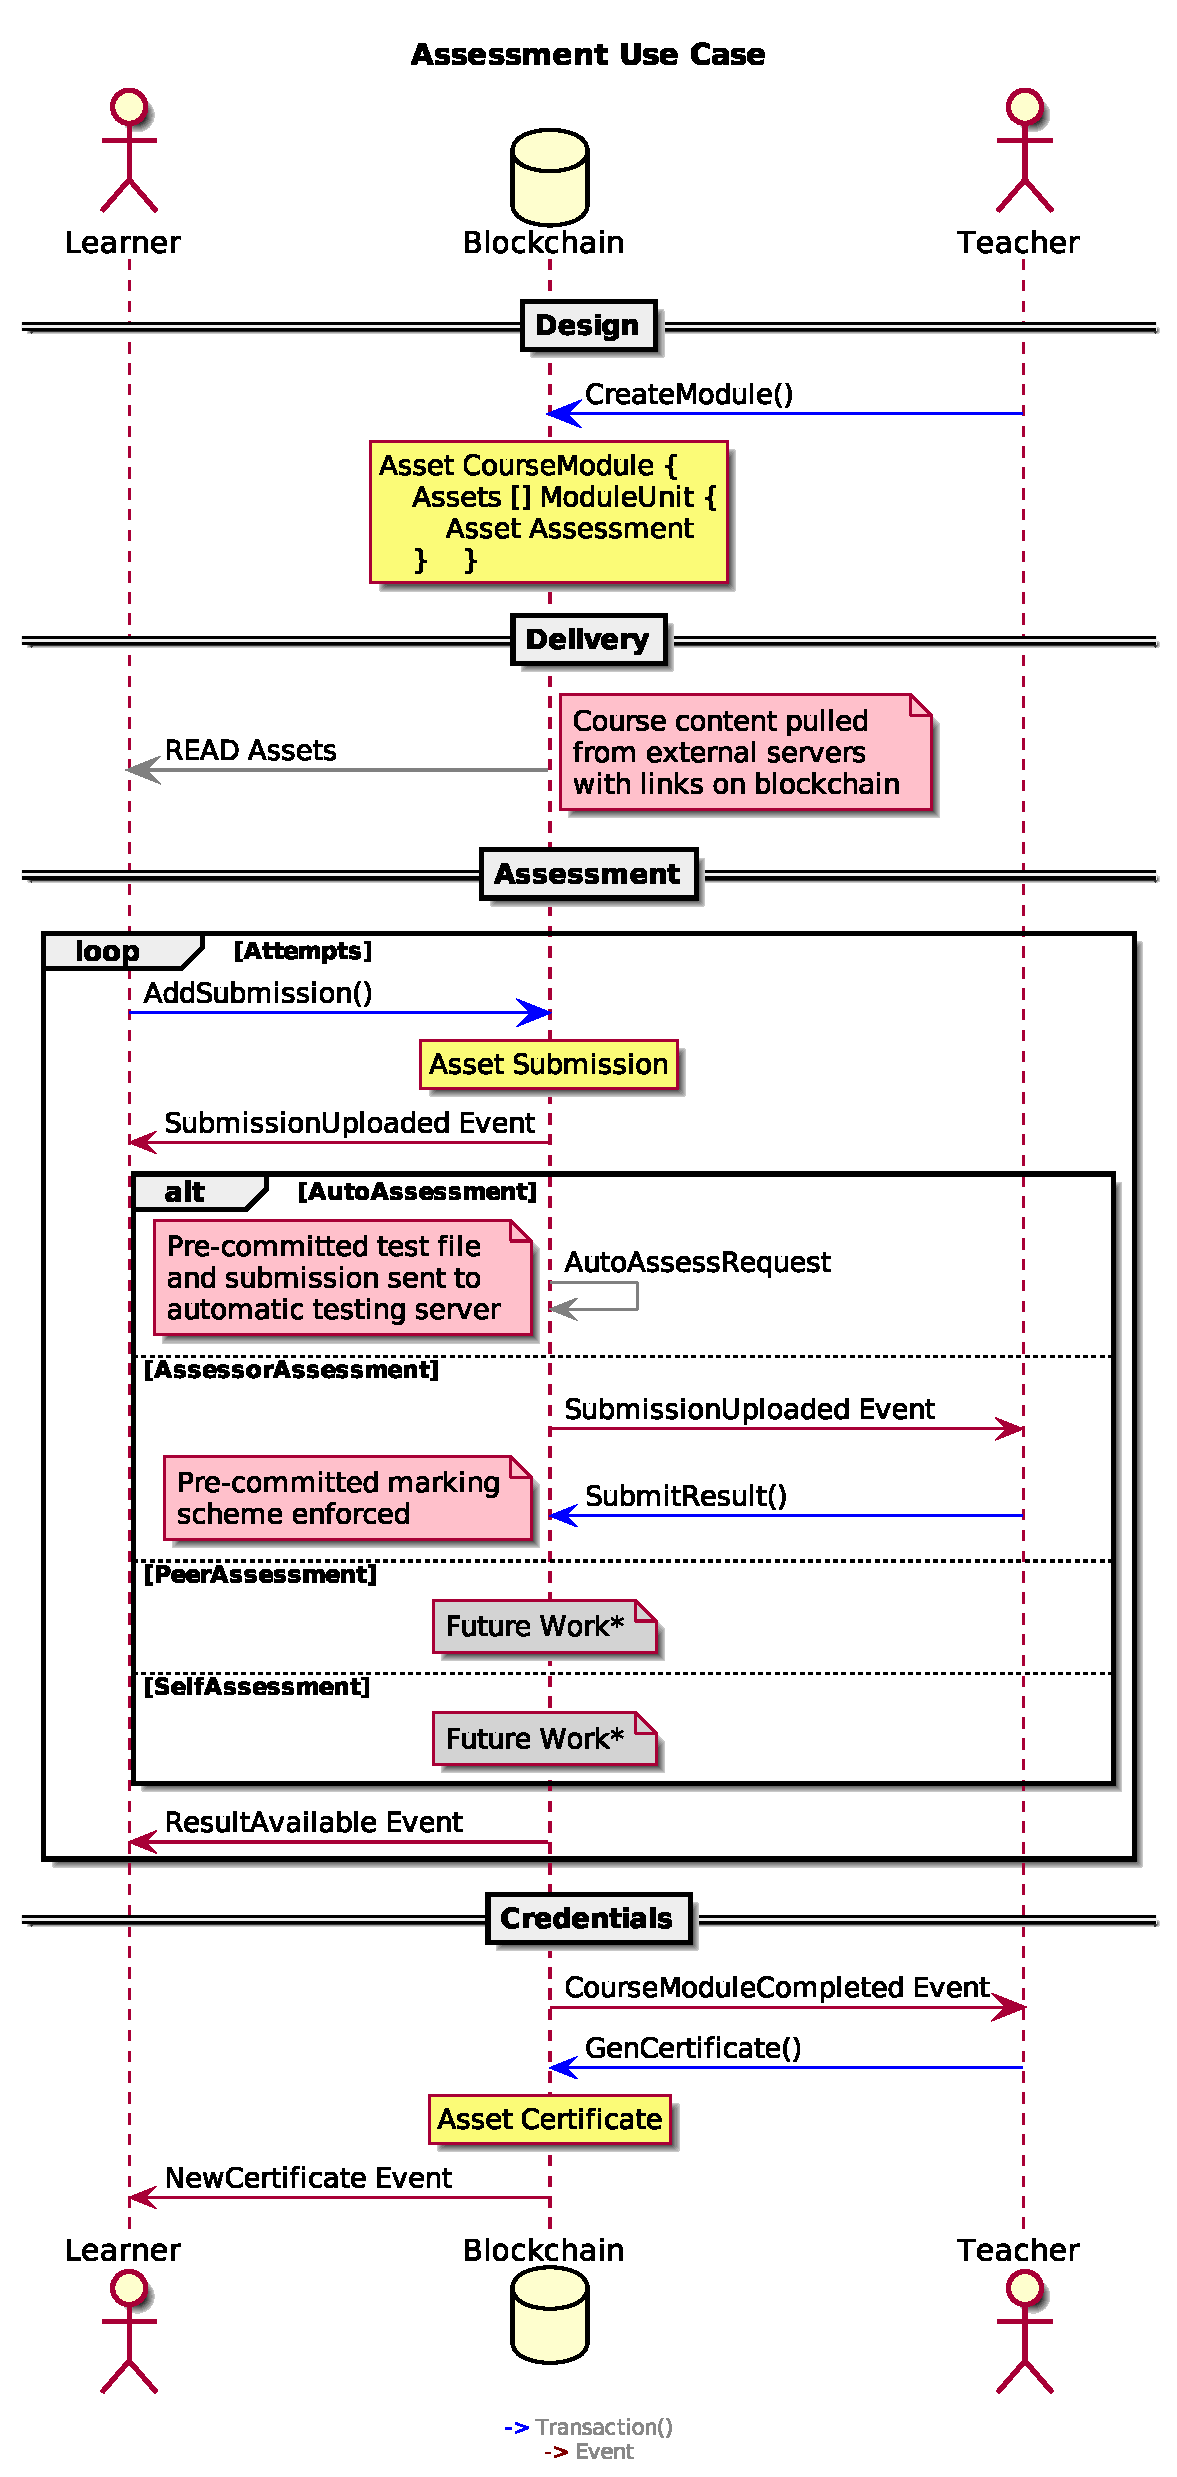
\includegraphics[width=0.65\textwidth]{assessmentloop}
	\caption[Assessment Use Case]
	{A UML sequence diagram denoting the assets, transactions and events between
		Learner and Teacher participants on the blockchain for the assessment use case}
	\label{fig:assessmentloop}
\end{figure}

\begin{itemize}
	\setlength\itemsep{0em}
	\item CreateModule: a transaction ordered by a teacher to store metadata about a course module,
	      its units and assessments onto the blockchain;
	\item AddSubmission: a transaction ordered by a learner to store a submission (assessment attempt)
	      on the blockchain, this could return the result of the assessment if the result is returned by
	      an automatic (machine) marking service;
	\item SubmitResult: a transaction ordered by a teacher to store details of an assessor assessment
	      for a submission on the blockchain;
	\item GenCertificate: a transaction ordered by a teacher to create a new certificate on the blockchain.
\end{itemize}

\subsection{Curriculum Personalisation Use Case}

Similarly, we looked at the transactions required to build a minimum viable product
that facilitates curriculum personalisation. A curriculum here is simply a list of course
modules attached to a learner and a teacher (a personal tutor for the learner).

\begin{itemize}
	\setlength\itemsep{0em}
	\item ProposeCurriculum: a transaction ordered by a learner or a teacher to propose
	      a new curriculum, or to proposed edits to an existing curriculum on the blockchain.
	\item ApproveCurriculum: a transaction ordered by a teacher to enrol a learner to
	      the course modules in the learner's curriculum.
\end{itemize}

See Figure \ref{fig:personalisationloop} for where these two transactions occur in a sequence diagram.

\begin{figure}[!ht]
	\centering
	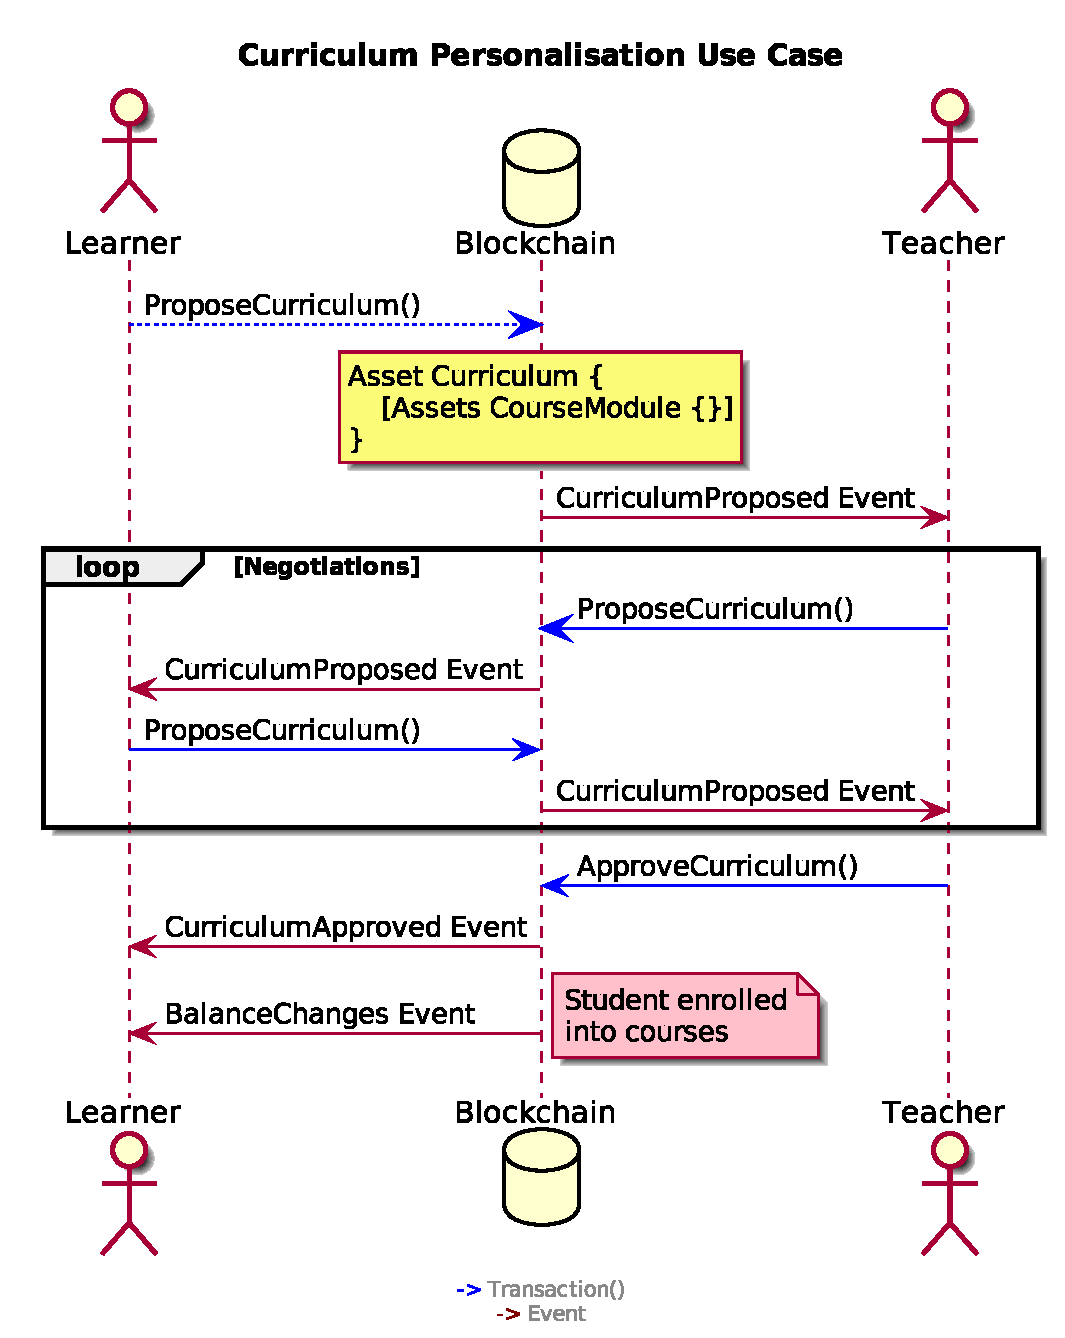
\includegraphics[width=0.7\textwidth]{personalisationloop}
	\caption[Curriculum Personalisation Use Case]
	{Sequence diagram denoting the assets, transactions and events between
		Learner and Teacher participants on the blockchain for the curriculum personalisation use case}
	\label{fig:personalisationloop}
\end{figure}

% automatic formative assessments Annette's student

% schema --> reviewer

\section{Data Models}

Building a blockchain network requires a network-wide schema of what records are allowed to be created, updated and read.
The Hyperledger Composer framework calls these resource definitions, and recommends defining objects
inheriting three basic types: Participants, Assets and Concepts in its object-oriented modelling language
\citep{official2018composer}.

\subsection{Participants}

A participant is an actor in a blockchain network. A participant can create and exchange other assets
by submitting transactions \citep{official2018composer}.
The network design for this project will allow the creation of three main types of participants:
\begin{itemize}
	\setlength\itemsep{0em}
	\item \textit{Teacher}, which can be lecturers, teaching assistants, tutors, etc.
	\item \textit{Learner}, which can be campus students, distant learners, etc.
	\item \textit{Reader}, members of the public who are interested in querying or verifying records,
	      such as employers and further education providers.
\end{itemize}

All three types of participants inherit an abstract (cannot be created) class \textit{User}. The \textit{nid} field
that all \textit{Users} must have would contain a one-way hash of their national identification number, which can be a
driver's license number, social security number, etc. A hash is a form
of cryptographical representation of data that is non-invertible. This allows the system to ensure that
all writers in the system is known and unique, while protecting their privacy to the general public.

See Figure \ref{fig:participants} for the detailed entity properties of all participant types
in a class diagram.

\begin{figure}[!ht]
	\centering
	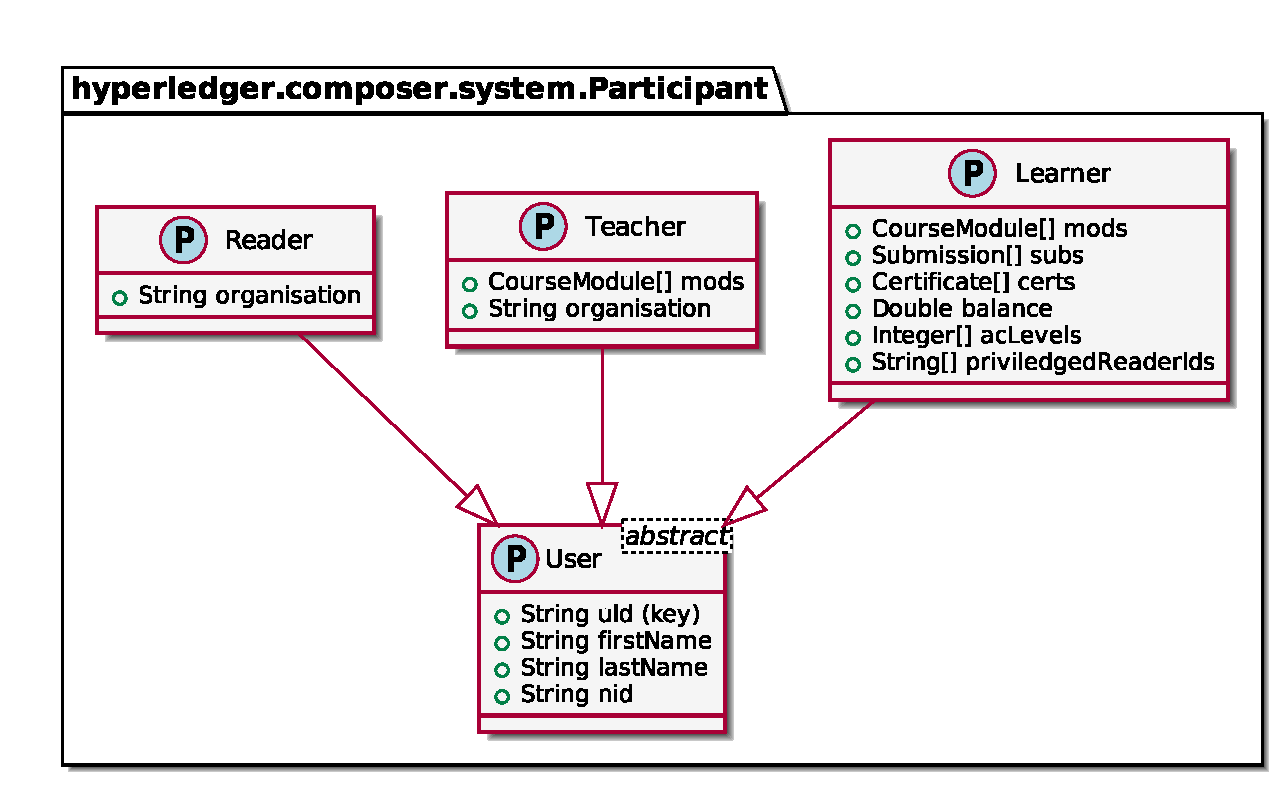
\includegraphics[width=0.7\textwidth]{participants}
	\caption[Participants Class Diagram]
	{A UML class diagram describing the participants defined on the blockchain}
	\label{fig:participants}
\end{figure}

A notable design consideration is the mechanism for allowing tiered access control of
learner information. The \textit{acLevels} and \textit{priviledgedReaderIds} fields in \textit{Learner}
store access control settings for two tiers of \textit{Readers}, normal and privileged.
This will be covered in more detail in an upcoming section.

\subsection{Assets}

Assets are "tangible or intangible goods, services, or property, and are stored in registries" \citep{official2018composer}.

\begin{figure}[!ht]
	\centering
	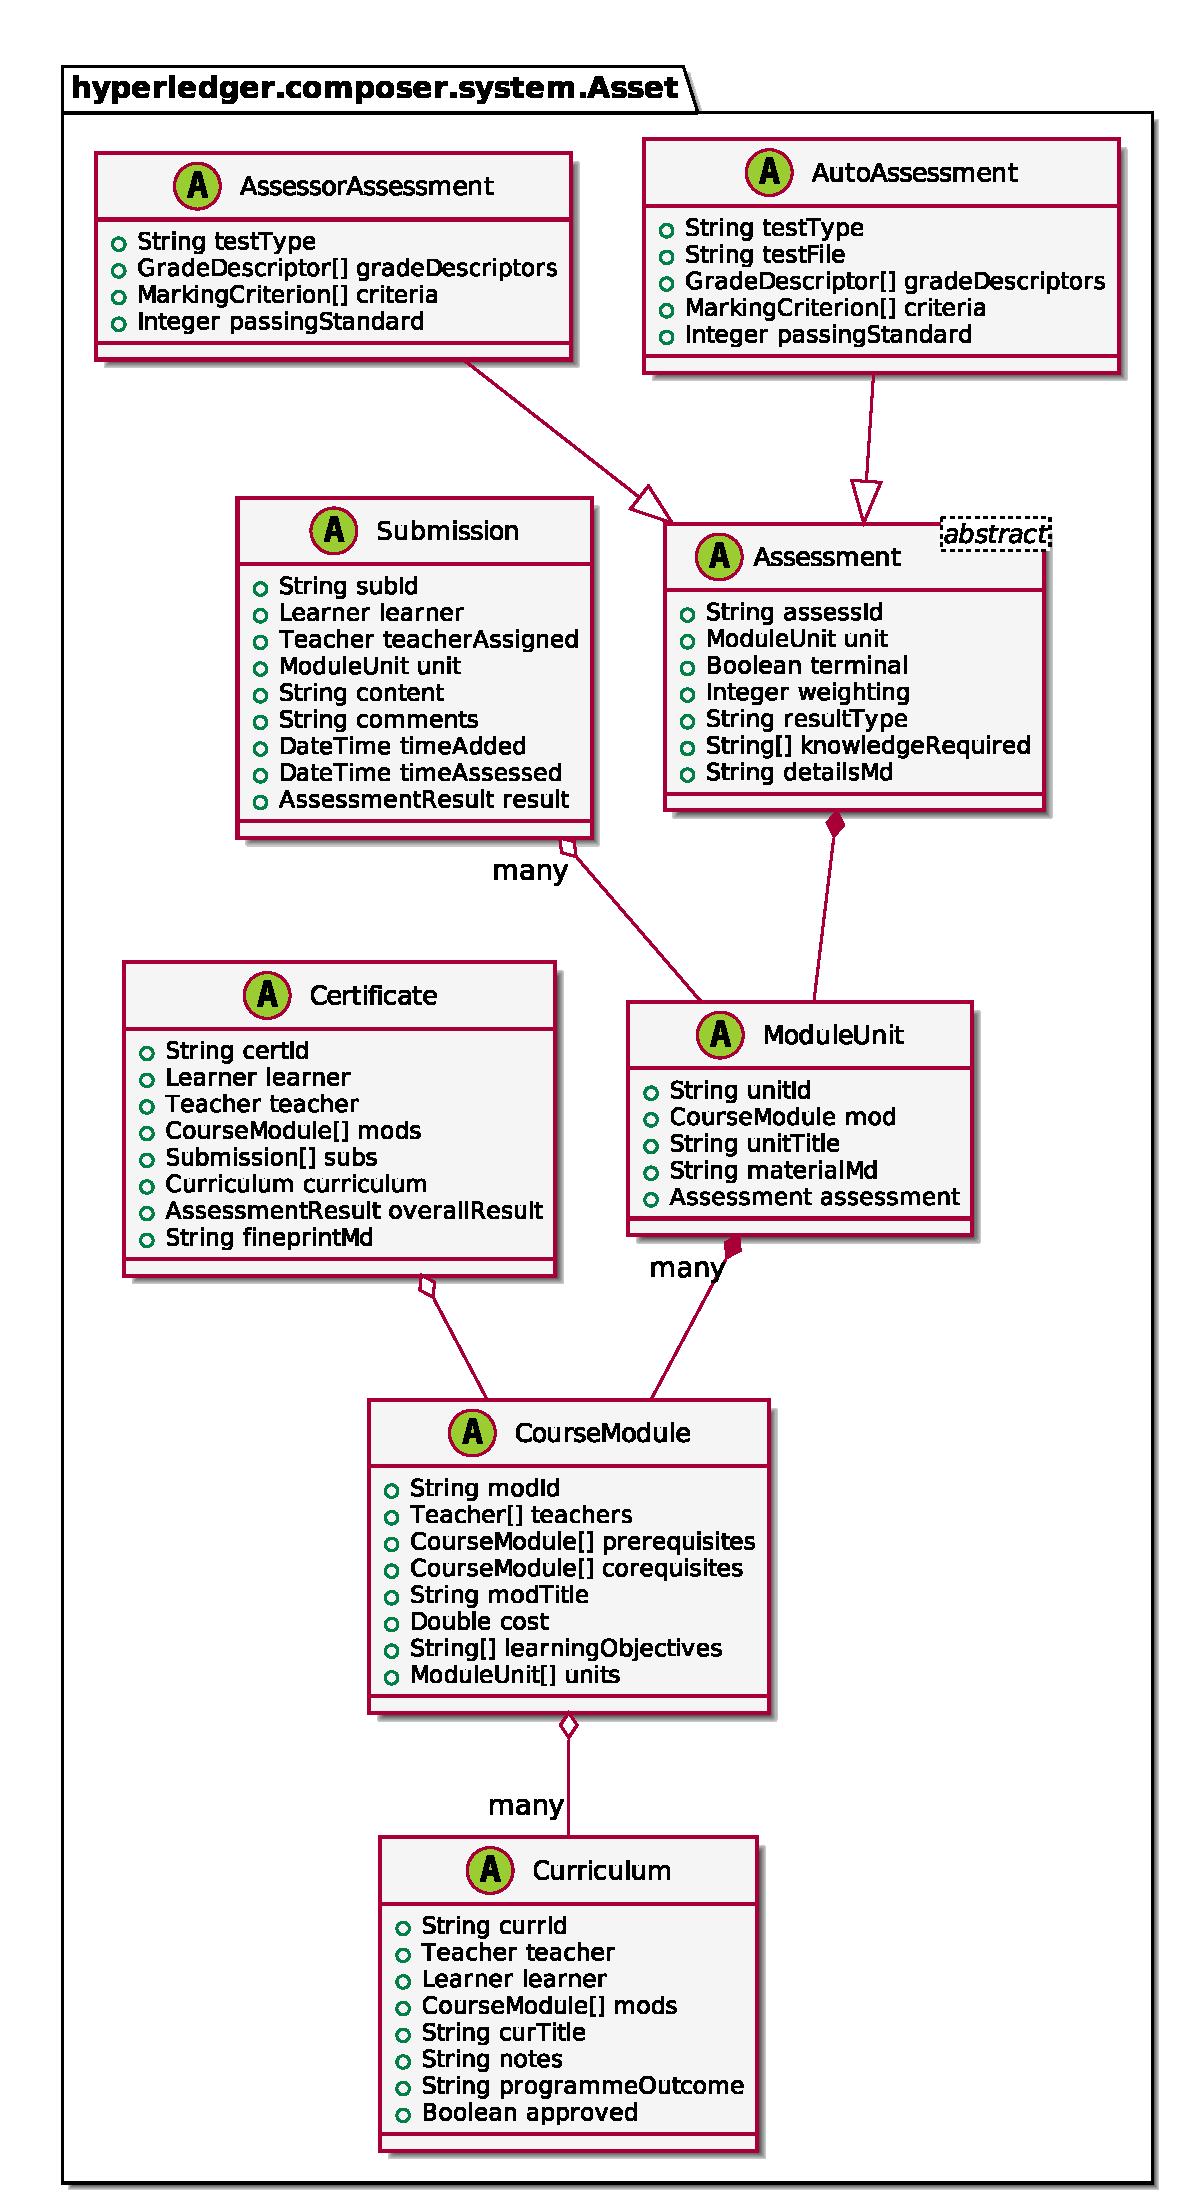
\includegraphics[width=0.6\textwidth]{assets}
	\caption[Assets Class Diagram]
	{A UML class diagram describing the assets defined on the blockchain}
	\label{fig:assets}
\end{figure}

See Figure \ref{fig:assets} for the detailed entity properties and relationships of these assets in a class diagram. 
The asset definitions are modelled carefully according to literature and user requirements.
The special design considerations included:

\begin{itemize}
	\setlength\itemsep{0em}
	\item \underline{Types of assessments}: A review of e-Learning and course management systems showed that online assessments could be
	      grouped in four categories: self assessment, computer assessment, tutor assessment, and peer assessment
	      \citep[p.68]{paulsen2004online}. In this initial design, two of these types are considered: \textit{AutoAssessment} (computer
	      assessment), and \textit{AssessorAssessment} (tutor assessment). They are daughter classes of the abstract \textit{Assessment}.
	\item \underline{Transparency of assessment goals}: the model contains mandatory fields to improve transparency in assessments, as identified by
	      \citet{suhre2013determinants}'s research reviewed in Chapter 2.1.1. This includes the \textit{knowledgeRequired} field
	      in \textit{Assessment} and \textit{learningObjectives} in \textit{CourseModule}, which encourage teachers to provide
	      clarity over assessment goals.
	\item \underline{Transparency of assessment procedures}: \textit{Assessment} assets are on the blockchain and visible to all participants,
	      improving transparency of procedures.
	      They include the \textit{gradeDescriptors} and \textit{criteria} fields that which encourage teachers to provide clarity of
	      assessment criteria, and give Smart Contracts the capabilities to enforce these criteria.
	\item \underline{Administrative Work for Personalisation}: Primary data suggested that administrative and regulatory work required for
	      curriculum personalisation could be daunting for institutions. The \textit{programmeOutcomes} field in the \textit{Curriculum} asset is one of
	      the suggested regulatory steps for the UK market (see Ch4.X TODO). Making these administrative data available on the blockchain
	      could allow future Smart Contracts to automate approvals and other administrative steps. This has the potential to reduce
	      bureaucracy by eliminating the middleman.
	\item \underline{Content flexibility}: It is anticipated that many markets, institutions, teams and teachers
	      will have their own requirements, formats and templates for what their e-Learning content should look like. To cater to
	      this need for content and layout flexibility the blockchain will accept markdown syntax as input in fields such as
	      \textit{detailsMd} in \textit{Assessment}, \textit{materialMd} in \textit{ModuleUnit} and \textit{fineprintMd} in \textit{Certificate}.
	      Markdown is a popular text-to-HTML conversion tool for web writers \citep{gruber2004markdown}, with many internet forums and
	      services releasing their own standards.
\end{itemize}

\subsection{Concepts}

Concepts are abstract classes that are not assets or participants. They are used to define custom properties contained by an asset or participant.

For this project: five of these Concepts were designed. These are related to modelling the assessment results, grade descriptors and criteria.
See figure \ref{fig:concepts} for their detailed entity properties.

\begin{figure}[!ht]
	\centering
	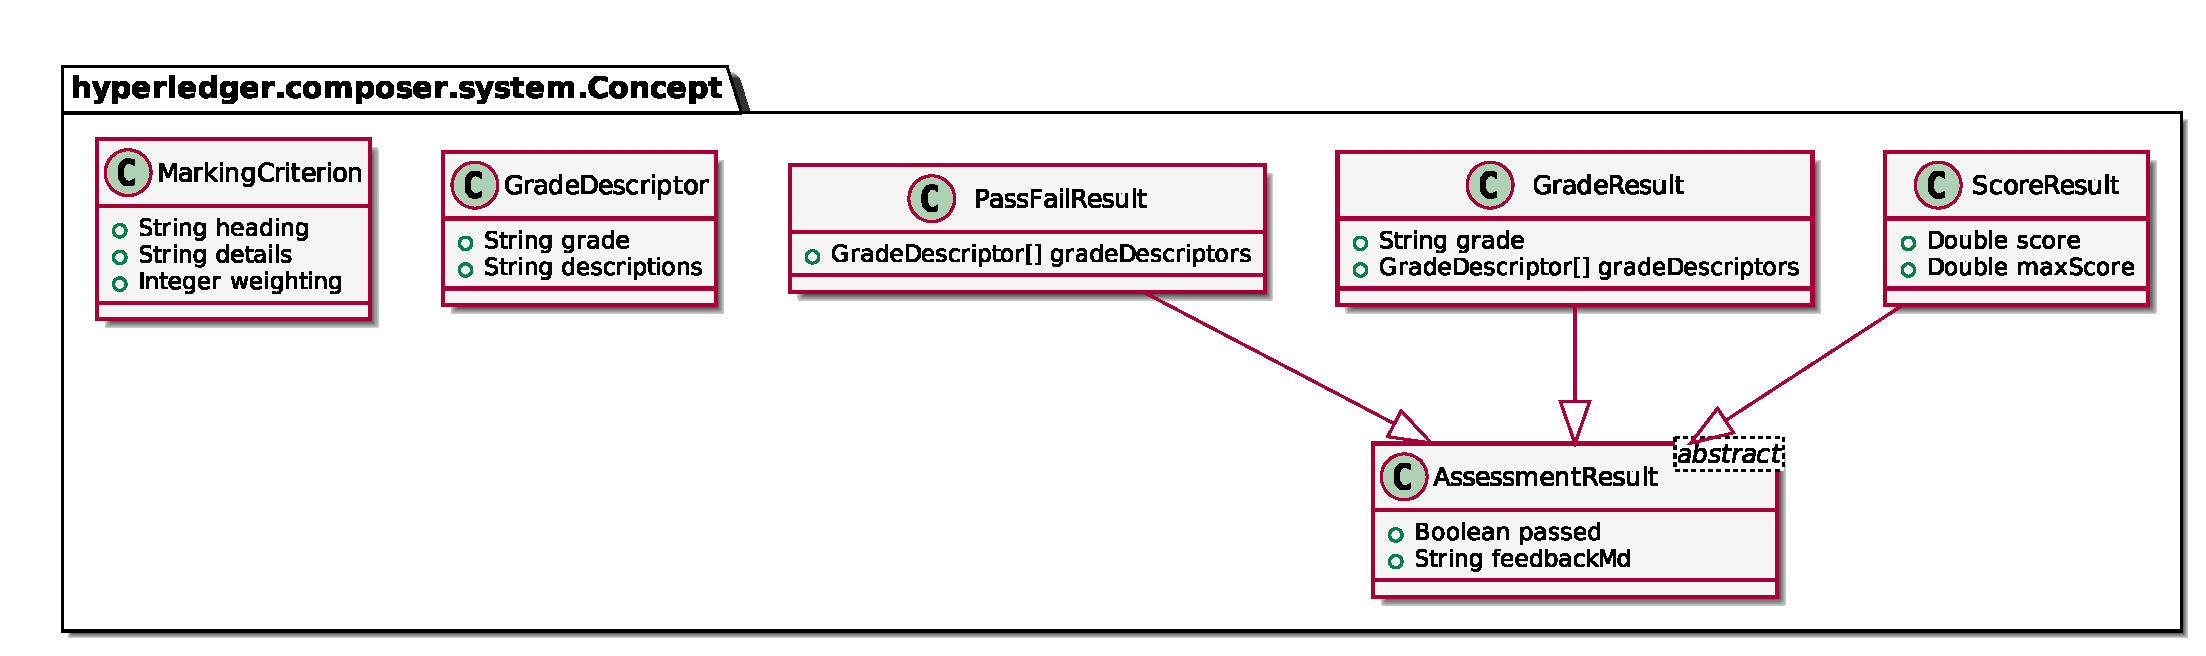
\includegraphics[width=1.0\textwidth]{concepts}
	\caption[Concepts Class Diagram]
	{A UML class diagram describing the concepts (other abstract classes that are contained as a field) defined on the blockchain}
	\label{fig:concepts}
\end{figure}

A matrix/ grid of assessment criteria against grade definitions, a common format used in schools \citep[p.102]{bryan2006innovative},
is used to record grade breakdowns on the blockchain. The \textit{MarkingCriterion} and \textit{GradeDescriptors} fields are designed to
fulfil this feature.

\textit{AssessmentResult} stores the overall result of an assessment or course module, as an example of how flexible this can be (TODO link to requirement),
three example result formats are designed: \textit{PassFailResult}, \textit{GradeResult}, and \textit{ScoreResult}.

\section{Smart Contracts: Transaction Logic and Events}

We have previously discussed the nature of Smart Contracts in Chapter 2.3.2. They are autonomous, self-sufficient and
decentralised code that runs on a blockchain.

In Hyperledger Composer, Smart Contracts are called chaincode.
They are run synchronously with a transaction order and a final output is required, to either accept the transaction, or reject it.
Smart Contract chaincode can emit network-wide Events. These Events could be consumed by participants or applications.

The discussion below describes the six transactions previously planned in Figure \ref{fig:assessmentloop} and \ref{fig:personalisationloop},
and the chaincode logic triggered by them.

\subsection{The CreateModule Transaction}

The transaction for creating a course module was kept simple, as this project is more interested in the assessment experience than the
content creation experience. A \textit{CourseModule} asset is uploaded with all of its \textit{ModuleUnits} and \textit{Assessments}.

\begin{figure}[!ht]
	\centering
	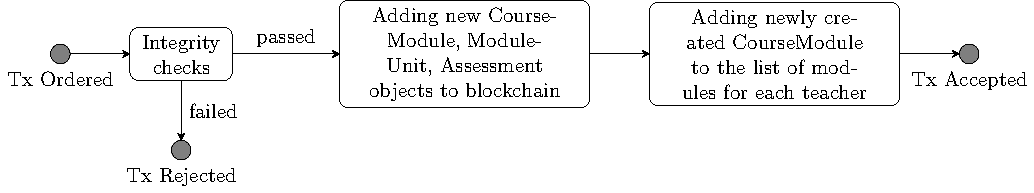
\includegraphics[width=1.0\textwidth]{cmtx}
	\caption[CreateModule Transaction flowchart]
	{Flowchart representation of the Smart Contract for the CreateModule Transaction (Tx)} \label{fig:cmtx}
\end{figure}

Transactions that allow content editing and course archiving (making courses unavailable to new students) will have to be designed
for a fully-fledged real world system, but we will defer them to future work for this project.

\subsection{The AddSubmission Transaction}

This transaction is ordered by a student to add a submission for the assessment of a module unit. The submission files will be
compressed and converted into base64 data strings and attached to the \textit{content} parameter.

\begin{figure}[!ht]
	\centering
	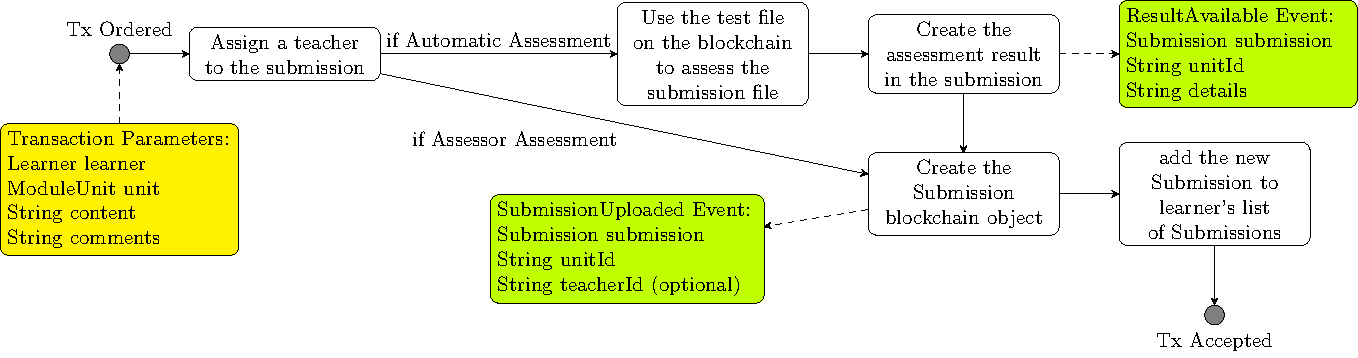
\includegraphics[width=1.0\textwidth]{astx}
	\caption[AddSubmission Transaction flowchart]
	{Flowchart representation of the Smart Contract for the AddSubmission Transaction (Tx)} \label{fig:astx}
\end{figure}

\subsection{The SubmitResult Transaction}

The assessor submits markings on a marking criteria against grade descriptor grid. This is uploaded as the transaction
parameter \textit{marks}, a one dimensional array where the index correlates to the marking criteria number and
the value correlates to the grade number.

\begin{figure}[!ht]
	\centering
	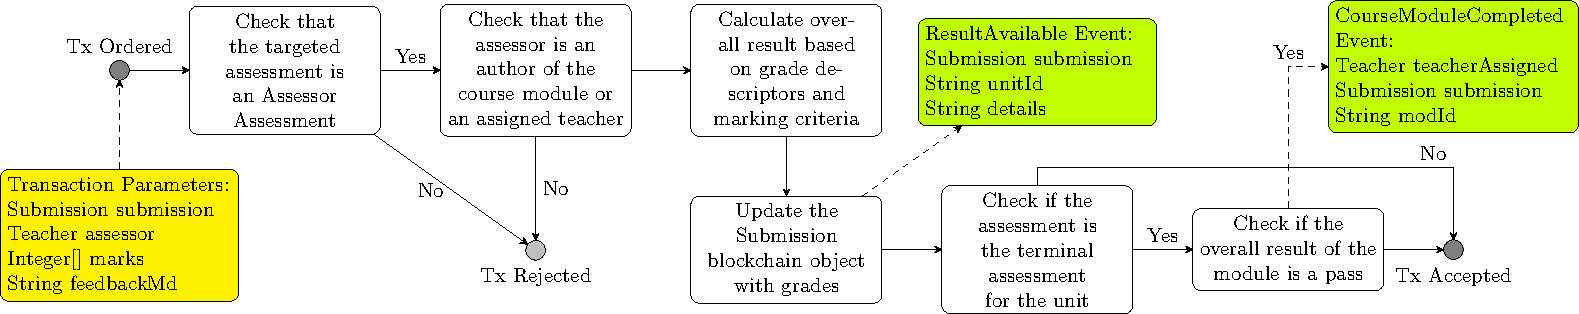
\includegraphics[width=1.0\textwidth]{srtx}
	\caption[SubmitResult Transaction flowchart]
	{Flowchart representation of the Smart Contract for the SubmitResult Transaction (Tx)} \label{fig:srtx}
\end{figure}

\subsection{The GenCertificate Transaction}

This transaction is designed to allow and encourage manual diligence over course completion evidences before issuing a certificate.
It could also require multiple signatures for a certificate.

\begin{figure}[!ht]
	\centering
	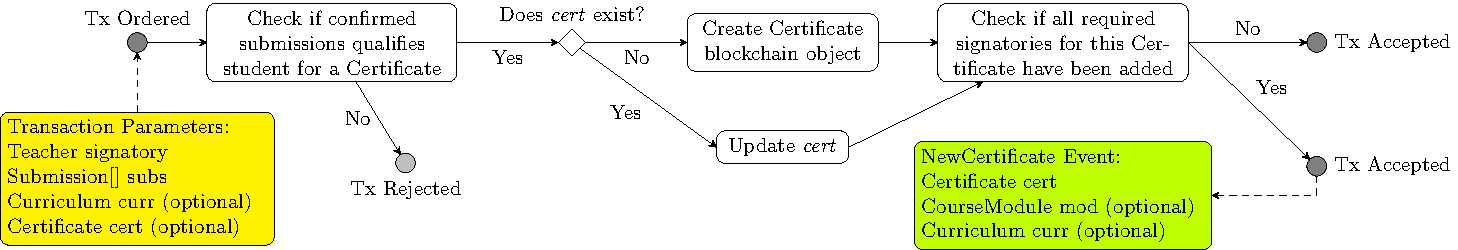
\includegraphics[width=1.0\textwidth]{gctx}
	\caption[GenCertificate Transaction flowchart]
	{Flowchart representation of the Smart Contract for the GenCertificate Transaction (Tx)} \label{fig:gctx}
\end{figure}

\subsection{The ProposeCurriculum Transaction}

\begin{figure}[!ht]
	\centering
	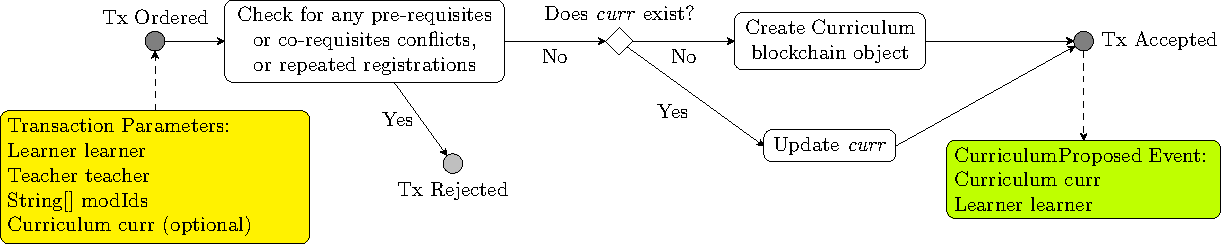
\includegraphics[width=1.0\textwidth]{pctx}
	\caption[ProposeCurriculum Transaction flowchart]
	{Flowchart representation of the Smart Contract for the ProposeCurriculum Transaction (Tx)} \label{fig:pctx}
\end{figure}

\subsection{The ApproveCurriculum Transaction}

\begin{figure}[!ht]
	\centering
	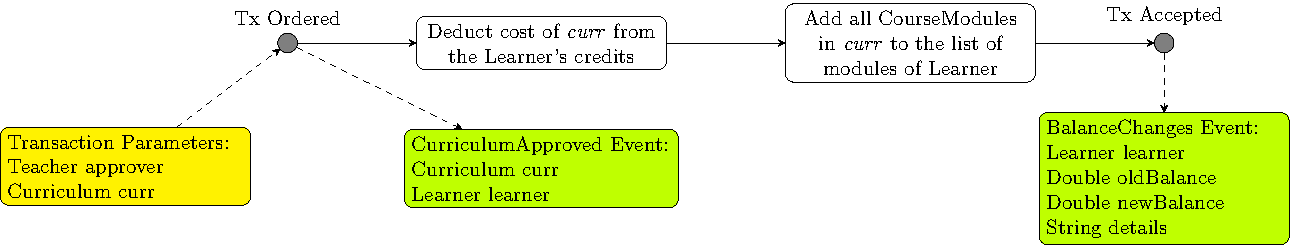
\includegraphics[width=1.0\textwidth]{actx}
	\caption[ApproveCurriculum Transaction flowchart]
	{Flowchart representation of the Smart Contract for the ApproveCurriculum Transaction (Tx)} \label{fig:actx}
\end{figure}

\section{Access Control}
The design of access control on the blockchain network is based on the Access Control Language of Hyperledger Composer.
It allows for the creation of access control rules that are conditional upon: the type of participant or asset,
the use of a specific transaction, and the values of properties of the participant or asset.

This means the mode of access control for the blockchain is both role-based and attribute-based.
Figure \ref{fig:ac_model} is a generic representation of what an access control rule deployed to the Hyperledger Fabric blockchain is composed of,
drawn based on the style proposed by \citet{poniszewska2005representation} for extended role-based access controls.\\

\begin{figure}[!ht]
	\centering
	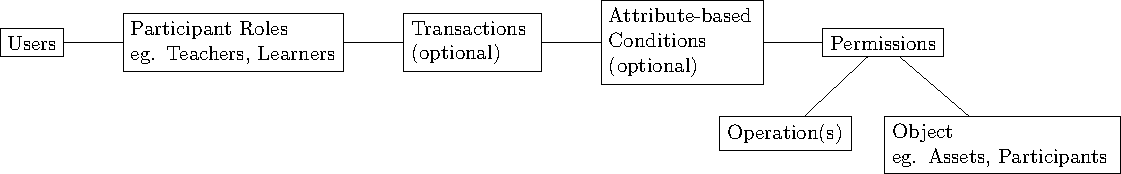
\includegraphics[width=1.0\textwidth]{ac_model}
	\caption[Access Control Model of Hyperledger Composer]
	{A flowchart representation of the Access Control model offered by Hyperledger Composer \citep{official2018composer}.}
	\label{fig:ac_model}
\end{figure}

Most of the rules are a form of Mandatory Access Controls across the network, enforced by the system and cannot be modified by
users or client applications, where access to objects is restricted based on fixed security attributes \citep{yuan2005attributed}.
Unless explicitly allowed by a defined access control rule, all operations are denied by default.

Some rules are more discretionary because the security-related attributes can be changed by users.
For example, a \textit{Learner} will be able to set its own \textit{acLevels} and \textit{priviledgedReaderIds} fields to control
what records related to the \textit{Learner} that \textit{readers} can read. Integer values are stored in \textit{acLevels} correlating to
a permission permutation model inspired by UNIX file permissions.

\begin{table}[!ht]
	\caption{The Reader access permutation model for Learner assets}
	\centering
	\label{table:reader_permutations}
	\begin{tabular}{|c|c|c|c|c|c|c|c|c|}
		\hline
		                     & 0 & 1          & 2          & 3          & 4          & 5          & 6          & 7          \\
		\hline
		Certificates         &   & \checkmark &            & \checkmark &            & \checkmark &            & \checkmark \\
		\hline
		Submissions          &   &            & \checkmark & \checkmark &            &            & \checkmark & \checkmark \\
		\hline
		Learner, Curriculums &   &            &            &            & \checkmark & \checkmark & \checkmark & \checkmark \\
		\hline
	\end{tabular}
\end{table}

So an \textit{acLevels} value of \texttt{[1, 3]} would mean all \textit{readers} can read your \textit{Certificates},
while \textit{readers} included in \textit{priviledgedReaderIds} can read your \textit{Certificates} and \textit{Submissions}.

Table \ref{table:ac_rules} lists all of the access control rules designed for the blockchain of this project.

\begin{landscape}
	\begin{table}[!ht]
		\caption{The access control rules designed for the blockchain}
		\centering
		\label{table:ac_rules}
		\begin{tabularx}{24cm}{l>{\hsize=.45\hsize}X>{\hsize=.55\hsize}X>{\hsize=0.9\hsize}Xc>{\hsize=.65\hsize}X}
			   & Role                     & Transaction                                   & Attribute-based Condition                                      & Operation(s)   & Object(s)                            \\
			\toprule
			1  & Learner, Teacher, Reader & --                                            & --                                                             & READ           & CourseModule, ModuleUnit, Assessment \\
			\midrule
			2  & Learner                  & --                                            & user.uId == object.uId                                         & UPDATE, READ   & Learner                              \\
			\midrule
			3  & Learner                  & --                                            & --                                                             & READ           & Teacher, Reader                      \\
			\midrule
			4  & Learner                  & AddSubmission                                 & user.uId == object.learner.uId                                 & CREATE         & Submission                           \\
			\midrule
			5  & Learner                  & --                                            & user.uId == object.learner.uId                                 & READ           & Submission                           \\
			\midrule
			6  & Learner                  & ProposeCurriculum                             & user.uId == object.learner.uId                                 & CREATE, UPDATE & Curriculum                           \\
			\midrule
			7  & Learner                  & --                                            & user.uId == object.learner.uId                                 & READ           & Curriculum                           \\
			\midrule
			8  & Teacher                  & --                                            & user.uId == object.uId                                         & UPDATE, READ   & Teacher                              \\
			\midrule
			9  & Teacher                  & --                                            & object.mods has (mod.teachers has (teacher.uId == user.uId))   & READ           & Learner                              \\
			\midrule
			10 & Teacher                  & --                                            & --                                                             & READ           & Reader                               \\
			\midrule
			11 & Teacher                  & CreateModule                                  & object.teachers has \newline(teacher.uId == user.uId)          & CREATE         & CourseModule, ModuleUnit, Assessment \\
			\midrule
			12 & Teacher                  & --                                            & object.unit.mod.teachers has \newline(teacher.uId == user.uId) & READ           & Submission                           \\
			\midrule
			13 & Teacher                  & SubmitResult                                  & user.uId == object.teacherAssigned.uId                         & UPDATE         & Submission                           \\
			\midrule
			14 & Teacher                  & --                                            & user.uId == object.teacher.uId                                 & READ           & Curriculum                           \\
			\midrule
			15 & Teacher                  & ProposeCurriculum, \newline ApproveCurriculum & user.uId == object.teacher.uId                                 & UPDATE         & Curriculum                           \\
			\bottomrule
		\end{tabularx}
	\end{table}
	(Continued on next page)
	\begin{table}
		\begin{tabularx}{24cm}{l>{\hsize=.45\hsize}X>{\hsize=.3\hsize}X>{\hsize=0.9\hsize}Xc>{\hsize=.65\hsize}X}
			   & Role   & Transaction & Attribute-based Condition                                                                   & Operation(s)           & Object(s)                                                                           \\
			\toprule
			16 & Reader & --          & user.uId == object.uId                                                                      & UPDATE, READ           & Reader                                                                              \\
			\midrule
			17 & Reader & --          & --                                                                                          & READ                   & Teacher                                                                             \\
			\midrule
			18 & Reader & --          & n = object.learner.acLevels[0]                                                              & READ*                  & Certificate (n>=1), \newline Submission (n>=3), \newline Learner, Curriculum (n>=5) \\
			\midrule
			19 & Reader & --          & object.learner.priviledgedReaderIds has (id == user.uId) AND n = object.learner.acLevels[1] & READ*                  & Certificate (n>=1), \newline Submission (n>=3), \newline Learner, Curriculum (n>=5) \\
			\midrule
			20 & ADMIN  & --          & --                                                                                          & CREATE, UPDATE, DELETE & PARTICIPANTS                                                                        \\
			\midrule
			20 & ADMIN  & --          & --                                                                                          & READ                   & ALL                                                                                 \\
			\bottomrule
		\end{tabularx}
	\end{table}

\end{landscape}

\section{Limitations}

Some limitations have been discovered for the above blockchain network design. They have not been accounted for or patched
because of either a desire to keep the design minimal and achievable, or a shortage of time to conduct background research.
Here is a list of the notable limitations:

\begin{itemize}
	\item The \textit{Teacher} participant was not designed to have different tiers of privileges. In higher education,
	      different roles such as module leader, module reviewer, supporting tutors exist. A module leader may also need the
	      permissions to create new \textit{Teacher} participants who are supporting tutors.
	\item There is no participant type for a higher education staff who is an institution administrator and not a teaching staff.
	      They may require more permissions than a regular \textit{Teacher} or \textit{Reader}, and bespoke transactions.
\end{itemize}

\section{User Interfaces for Client Applications}

To demonstrate the improvements a blockchain back-end and Smart Contracts can bring to an e-Learning platform, a
Learner client application and a Teacher client application will be built at the implementation stage.

While improving general usability is not one of the objectives of this project, poor usability and interface designs
could adversely affect evaluation of the improvements that this project aims for.

Therefore, several of \citet{nielsen199510}'s famous five usability design goals and ten usability design hieuristics
were considered when developing the application prototypes. See Table \ref{table:ux_considerations}:

\begin{table}[!ht]
	\caption{Usability considerations for client applications}
	\centering
	\label{table:ux_considerations}
	\begin{tabularx}{\textwidth}{lXX}
		Usability Goal            & Usability Hieuristic                                    & Example Non-functional requirements    \\
		\toprule
		Learnability              & Match between system and the real world\newline
		Visibility of system status \newline
		Consistency and standards & Using common higher education glossary \newline
		Notifications Area \newline
		Adopt a popular design language                                                                                              \\
		\midrule
		Efficiency                & Flexibility and efficiency of use                                                                \\
		\midrule
		Memorability              & Recognition rather than recall                          & Always Visible Navigation Menu         \\
		\midrule
		Error Reduction        & Help users recognize, diagnose, and recover from errors & Error Messages on Transaction Failures \\
		\midrule
		Satisfaction              & Aesthetic and minimalist design                                                                  \\
		\bottomrule
	\end{tabularx}
\end{table}

To maximise learnability and user familiarity, the client applications will adopt a popular design language for their user interfaces.
Material Design, a design system that combines theory, resources, and tools, is used by the most popular mobile operating system Android 
and many web applications \citep{google2018material}. Resources such as free-to-use icon packs and tools such as well-maintained 
user interface component libraries on various mobile and web development platforms will enable quick scaffolding of design compliant and 
highly usable applications.

Figure \ref{fig:sitemaps} are the sitemap trees showing the contextual flow for users in the client applications:

\begin{figure}[!ht]
	\centering
	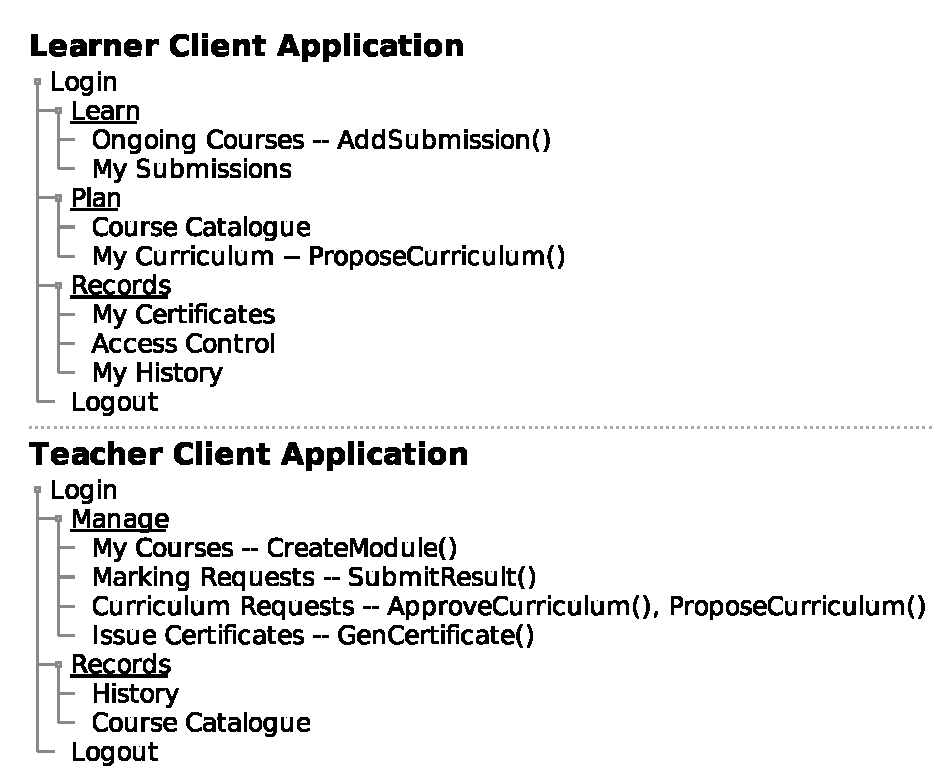
\includegraphics[width=.6\textwidth]{sitemaps}
	\caption[Client Application Sitemaps]
	{Sitemap designs for the learner and teacher client applications with notes on the location of transaction ordering dialogues.} \label{fig:sitemaps}
\end{figure}

No low fidelity prototypes for the two demonstrator applications were produced due to the lack of research need, 
since the usability design was driven by hieuristics and not a more user-centred approach. The next chapter will 
describe further how high fidelity, demonstration-ready web applications were built for this project.